% ISY5004 Final Report
% Style: spconf.sty (ICASSP/ICIP), IEEEbib.bst
\documentclass{article}
\usepackage{spconf,amsmath,graphicx}
\usepackage{booktabs}
\usepackage{subcaption}
\usepackage{url}
\usepackage{array}

\graphicspath{{figures/}}

% Title
\title{Do Self-Supervised Vision Models Learn What Experts See?}

\name{Desmond Choy, Leong Kay Mei}
\address{NUS-ISS, National University of Singapore, Singapore 119615}

\begin{document}
%\ninept
\maketitle

\begin{abstract}
Self-supervised vision models achieve strong downstream performance, but high
classification accuracy alone does not reveal whether those models attend to the
same visual evidence that human experts consider diagnostically important. This
project studies that question in the WikiChurches setting, where expert bounding
boxes identify architectural features such as arches, windows, towers, and
facade elements that matter for style recognition. We evaluate seven vision
models across self-distillation, masked autoencoding, multimodal contrastive
pretraining, and a supervised CNN baseline, then measure attention alignment
against 631 expert boxes on 139 annotated church images using IoU, Coverage,
MSE, KL divergence, and EMD. The study is organised around three linked
questions: how well frozen models align with expert-marked regions, how Linear
Probe, LoRA, and Full fine-tuning change that alignment, and whether individual
attention heads exhibit descriptive specialisation for different architectural
features. For Q1, DINOv3 provides the strongest frozen alignment, leading on
IoU, Coverage, KL, and EMD and clearing all calibrated naive baselines. For Q2,
fine-tuning effects are model-family dependent: CLIP gains the most
(IoU $0.0181\!\to\!0.0745$, Cohen's $d\!\approx\!1.0$) with gains concentrated
on Gothic and Romanesque features, MAE shows a large Renaissance shift driven by
pediment geometry, and the DINO family largely preserves its strong frozen
alignment. Models with different pretraining objectives converge on the same
structurally easy images rather than complementary subsets.
\end{abstract}

\textbf{Keywords}: self-supervised learning, attention alignment, vision transformers, architectural recognition

% -----------------------------------------------------------------------
\section{Introduction}
\label{sec:intro}

A vision model can be correct for the wrong visual reasons. In architectural
style recognition, a model that classifies a church as Gothic because it attends
to pointed arches and flying buttresses is qualitatively different from one that
succeeds because it exploits background regularities or photographer bias
unrelated to expert reasoning. Accuracy alone cannot distinguish those cases.

WikiChurches~\cite{Barz21WikiChurches} provides a strong evaluation setting
because it pairs fine-grained architectural-style labels with expert bounding
boxes marking characteristic visual features, making it possible to compare
model attention directly against human expert targets rather than inferring
plausibility from class predictions alone.

This report addresses three linked research questions. \textbf{Q1}: Do frozen
SSL and baseline vision models attend to the same architectural regions that
experts mark as diagnostically important? \textbf{Q2}: How does attention change
after adaptation (Linear Probe, LoRA, Full fine-tuning), and does strategy
matter? \textbf{Q3}: Do individual attention heads exhibit descriptive
specialisation for different architectural features, and do dominant heads shift
across variants?

Taken together, these questions shift the project from a visualisation exercise
into a domain-grounded evaluation study of what different pretraining and
adaptation choices encourage models to attend to.

% -----------------------------------------------------------------------
\section{Literature Review}
\label{sec:lit}

\subsection{Attention Interpretability in Vision Transformers}

DINO~\cite{Caron21DINO} popularised the observation that late-layer
self-attention can resemble semantic object masks, while attention
rollout~\cite{Abnar20Rollout} argued that single-layer raw attention may miss
cross-layer information flow. Chefer et al.~\cite{Chefer21Interp} further
demonstrated that attention visualisation alone is not a complete explanation
method, which is why this project frames outputs as alignment measurements and
descriptive evidence rather than definitive causal proof.

\subsection{Evaluation Against Expert Annotations}

IoU-style localisation evaluation, pointing-game metrics, and
plausibility-oriented benchmarks~\cite{Zhou16CAM,Zhang16Excitation,Choe20Localization}
established the pattern of comparing model-derived maps against annotated
regions. Recent work in medical imaging~\cite{Chung25MedViT} found that model
families behave differently when the evaluation target is domain-specific,
strengthening the framing of this project as a domain-grounded evaluation study.

\subsection{Fine-Tuning, Representation Shift, and Attention Drift}

Kumar et al.~\cite{Kumar22Distort} showed that fine-tuning can distort
pretrained features relative to linear-probe controls.
Biderman et al.~\cite{Biderman24LoRA} argued that LoRA tends to learn less and
forget less than full fine-tuning. Park et al.~\cite{Park23SSLViT} and
Li et al.~\cite{Li24AttnTransfer} suggest that attention patterns are not
incidental to downstream performance and can be transferred usefully.

\subsection{Attention-Head Specialisation}

Voita et al.~\cite{Voita19Heads} established that only a subset of heads carries
the most interpretable behaviour. Later ViT work~\cite{Li23HeadDist,Walmer23Teaching,Raghu21ViTvsCNN}
extended that intuition to head-level spatial patterns. Q3 adopts this
descriptive framing: it asks whether some heads align more strongly with
architectural features, not whether the full model decision reduces to a single
head.

\subsection{Cultural Heritage and Architectural Recognition}

Architectural heritage datasets are appropriate for attention-alignment studies
because diagnostic evidence is structural, expert-defined, and visually
localised. The project's novelty lies in bringing together
expert-annotation-grounded evaluation, multiple SSL
paradigms~\cite{Caron21DINO,Oquab24DINOv2,Simeoni25DINOv3,He22MAE,Radford21CLIP,Zhai23SigLIP,Tschannen25SigLIP2},
adaptation analysis, and an architecture domain where looking at the right
evidence is central~\cite{Hu25ASCENT}.

% -----------------------------------------------------------------------
\section{Proposed Approach}
\label{sec:approach}

\begin{figure*}[t]
\centering
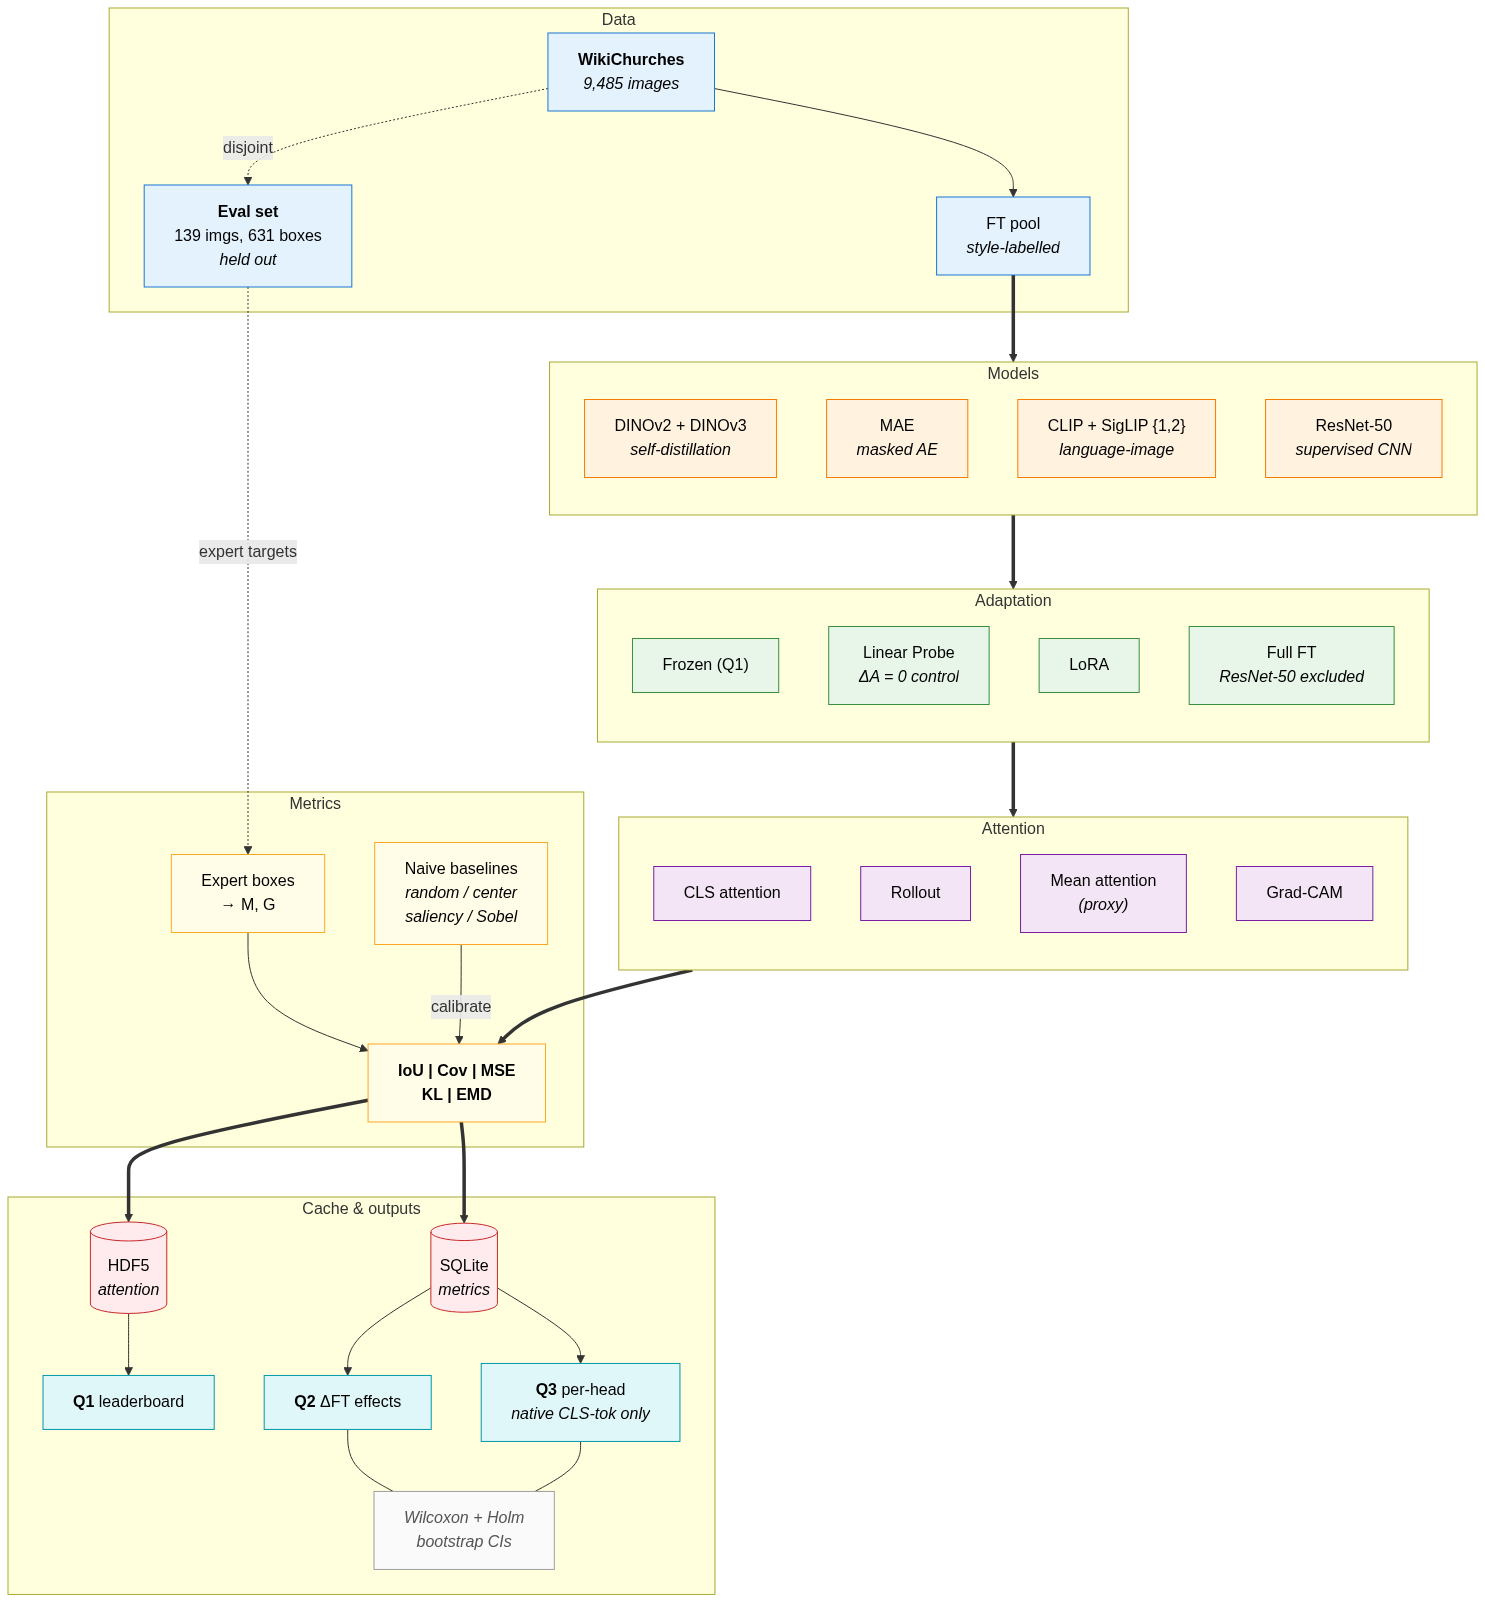
\includegraphics[width=0.95\textwidth]{pipeline.png}
\caption{End-to-end pipeline. The 139-image expert-annotated evaluation set is disjoint from the fine-tuning pool. Linear Probe is a zero-$\Delta$ control (backbone frozen); ResNet-50 is excluded from Q2. Attention extraction depends on model family; Q3 is restricted to native CLS-token models. Five alignment metrics are computed against expert boxes ($M$ binary, $G$ Gaussian) and calibrated against four naive baselines. Cached artefacts feed the Q1, Q2, and Q3 analyses.}
\label{fig:pipeline}
\end{figure*}

Figure~\ref{fig:pipeline} summarises the end-to-end pipeline. The remainder of
this section walks through each stage in turn.

\subsection{Dataset and Problem Setup}

The primary dataset is WikiChurches~\cite{Barz21WikiChurches}, a fine-grained
architectural-style dataset of European church buildings. The annotation file
defines 106 feature types (arches, windows, towers, portals, etc.) with
bounding boxes in normalised coordinates. This project uses two data scopes:
(1)~an expert-annotated evaluation subset of 139 images with 631 bounding boxes
(Romanesque~51, Gothic~49, Renaissance~22, Baroque~17), and (2)~a larger
style-labelled pool from the 9,485-image official release used for fine-tuning.
The 139 annotated images are held out from all fine-tuning splits.

A key caveat is \textit{sparse annotation bias}: WikiChurches annotates
representative instances rather than every visible occurrence of a feature, so
a model attending to multiple correct instances may still be penalised by IoU.
This is treated as a documented limitation rather than a pipeline defect.

\subsection{Models and Attention Extraction}

The frozen benchmark compares seven models: six ViT-Base transformers
(DINOv2~\cite{Oquab24DINOv2}, DINOv3~\cite{Simeoni25DINOv3},
MAE~\cite{He22MAE}, CLIP~\cite{Radford21CLIP}, SigLIP~\cite{Zhai23SigLIP},
SigLIP2~\cite{Tschannen25SigLIP2}) and ResNet-50 as a supervised CNN baseline.
DINOv2 uses patch size~14 with 4 register tokens ($16\!\times\!16$ spatial
grid); all others use patch size~16 ($14\!\times\!14$ grid).

Attention extraction depends on architecture (Table~\ref{tab:extraction}). CLS
attention and rollout are used for DINOv2, DINOv3, MAE, and CLIP. SigLIP and
SigLIP2 use a mean-attention proxy because they lack an equivalent CLS-token
pathway. ResNet-50 uses Grad-CAM. These distinctions are especially important
in Q3, which is restricted to architecture-native CLS-token models.

\begin{table}[h]
\caption{Attention extraction methods by model family.}
\label{tab:extraction}
\centerline{
\begin{tabular}{lll}
\toprule
Method & Models & Notes \\
\midrule
CLS attention & DINOv2, DINOv3, MAE, CLIP & Native CLS token \\
Rollout & DINOv2, DINOv3, MAE, CLIP & Cross-layer composition \\
Mean attention & SigLIP, SigLIP2 & Proxy (no CLS token) \\
Grad-CAM & ResNet-50 & CNN baseline \\
\bottomrule
\end{tabular}
}
\end{table}

\subsection{Alignment Metrics}

Five metrics are used because no single score suffices for all interpretations.
Let $A$ denote the attention heatmap, $M$ the union binary mask of expert boxes,
and $G$ a Gaussian soft-union target derived from the boxes.

\textbf{IoU} thresholds $A$ at the exact top-$k$ pixel count via
\texttt{torch.topk} (top~10\% of pixels) and computes overlap with $M$:
\begin{equation}
  \text{IoU} = \frac{|\hat{A} \cap M|}{|\hat{A} \cup M|}, \quad
  \hat{A} = \text{top-}k\text{-pixels}(A).
\end{equation}
Higher is better.

\textbf{Coverage} is threshold-free: the fraction of total attention energy
inside $M$,
\begin{equation}
  \text{Coverage} = \frac{\sum_{i \in M} A_i}{\sum_i A_i}.
\end{equation}
Higher is better.

\textbf{MSE}, \textbf{KL divergence}, and \textbf{EMD} compare the full
normalised heatmap against $G$. Lower is better for all three.

\subsection{Baselines and Calibration}

Continuous metrics are calibrated against four naive baselines: random
attention, center Gaussian, saliency prior, and Sobel edge map
(Table~\ref{tab:baselines}). Beating random only is weak evidence; clearing
all four baselines is stronger support for non-trivial semantic alignment.

\begin{table}[h]
\caption{Dataset-level naive baseline scores (lower is better).}
\label{tab:baselines}
\centerline{
\begin{tabular}{lccc}
\toprule
Baseline & MSE & KL & EMD \\
\midrule
Random         & 0.0223 & 3.9182 & 0.3468 \\
Center Gaussian & 0.0193 & 3.7124 & 0.3312 \\
Saliency Prior & 0.0189 & 3.6841 & 0.3298 \\
Sobel Edge     & 0.0201 & 3.8003 & 0.3401 \\
\bottomrule
\end{tabular}
}
\end{table}

\subsection{Fine-Tuning Protocol}

Q2 uses a shared experiment-batch workflow. Training is on the non-annotated
style-labelled pool with one stratified validation split shared across all
model$\times$strategy runs. Best checkpoints are selected by classification
validation accuracy; alignment is re-evaluated on the held-out annotated subset.
Three strategies are compared (Table~\ref{tab:strategies}); ResNet-50 is
excluded from Q2.

\begin{table}[h]
\caption{Fine-tuning strategies compared in Q2.}
\label{tab:strategies}
\centerline{
\begin{tabular}{lll}
\toprule
Strategy & Backbone & Role \\
\midrule
Linear Probe & Frozen & Control (zero attention change) \\
LoRA         & Mostly frozen & Efficient adapter \\
Full         & Updated end-to-end & Maximum adaptation \\
\bottomrule
\end{tabular}
}
\end{table}

\subsection{Per-Head Scope (Q3)}

Q3 is scoped to architecture-native CLS-token models: DINOv2, DINOv3, MAE,
and CLIP, with frozen, LoRA, and Full as the primary variants. Linear Probe is
a control. SigLIP, SigLIP2, and ResNet-50 are excluded because per-head
analysis for them relies on a proxy rather than native attention heads. Q3 is a
descriptive head-specialisation analysis, not a causal attribution method.

\subsection{Statistical Analysis}

The study uses paired t-tests, Wilcoxon signed-rank tests, bootstrap confidence
intervals, Cohen's $d$ for paired differences, and Holm multiple-comparison
correction. This is especially important in Q2, where many
model$\times$strategy$\times$metric combinations are compared within shared
correction families.

% -----------------------------------------------------------------------
\section{Experimental Results}
\label{sec:results}

\subsection{Dataset}

The 139-image annotated evaluation set spans four architectural styles. Average
expert boxes per image are 4.5 overall, but vary by style: Gothic and
Romanesque images are more densely annotated (4.2--5.9 boxes/image) than
Baroque images (1.8 boxes/image), which limits statistical power for that
subset.

\subsection{Implementation Details}

All ViT models use ViT-Base scale. Fine-tuning used AdamW with cosine learning
rate scheduling, early stopping on validation accuracy. LoRA adapters are
inserted into attention projection layers. Heatmaps are computed at a
standardised resolution and cached to HDF5/SQLite for fast backend serving.

\subsection{Performance Metrics}

Metrics are defined in Section~\ref{sec:approach}. IoU@90 denotes IoU at the
top-10\% pixel threshold. Directions: higher is better for IoU and Coverage;
lower is better for MSE, KL, and EMD. Results are reported at each model's
best default-method layer over the 139 annotated images.

\subsection{Q1: Frozen-Model Attention Alignment}

Table~\ref{tab:q1} ranks seven models by IoU@90 at their best default-method
layer. DINOv3 leads on IoU@90, Coverage, KL, and EMD, and is the only model
that clears all four naive baselines on all three continuous metrics. ResNet-50
ranks second on the two overlap metrics (IoU, Coverage), showing that supervised
CNN representations carry meaningful localisation behaviour even without
transformer attention. DINOv2 provides the stronger distributional second-tier
story among transformers (second on KL and EMD), consistent with
self-distillation producing more object-like late-layer attention.

CLIP is especially informative as a contrast: its best frozen IoU occurs at
layer~0 rather than in a late-layer regime, suggesting the language-image
contrastive objective does not inherently produce expert-aligned spatial
structure at depth. The SigLIP family achieves the best frozen MSE (0.0175) but
has EMD~0.3538, worse than the random baseline (0.3468), showing the danger of
single-metric interpretation: smooth local maps can still misplace attention
mass at a distributional level.

\begin{table}[h]
\caption{Q1 frozen-model alignment leaderboard (best default-method layer, 139 images). $\uparrow$ higher is better; $\downarrow$ lower is better.}
\label{tab:q1}
\centerline{\small
\begin{tabular}{llccccc}
\toprule
Model & Paradigm & IoU$\uparrow$ & Cov$\uparrow$ & MSE$\downarrow$ & KL$\downarrow$ & EMD$\downarrow$ \\
\midrule
DINOv3   & Self-distil. & \textbf{0.104} & \textbf{0.241} & 0.0182 & \textbf{3.412} & \textbf{0.318} \\
ResNet-50 & Supervised  & 0.089 & 0.198 & 0.0195 & 3.701 & 0.334 \\
DINOv2   & Self-distil. & 0.078 & 0.183 & 0.0188 & 3.524 & 0.321 \\
MAE      & Masked recon. & 0.061 & 0.159 & 0.0194 & 3.682 & 0.341 \\
CLIP     & Lang.-image  & 0.031 & 0.092 & 0.0209 & 3.687 & 0.410 \\
SigLIP   & Sigmoid CL   & 0.024 & 0.071 & \textbf{0.0175} & 3.651 & 0.354 \\
SigLIP2  & Sigmoid CL   & 0.023 & 0.069 & \textbf{0.0175} & 3.638 & 0.354 \\
\bottomrule
\end{tabular}
}
\end{table}

The absolute IoU values should not be read like classification accuracy. Because
annotations are sparse and often cover much less than 10\% of the image, even
strong spatial correspondence does not produce IoU near~1.0. The calibrated
interpretation is that DINOv3 is well ahead of other frozen models on overlap,
clears the strongest continuous-baseline tests, and remains statistically
separated from the next-best model (paired Wilcoxon, Holm-corrected $p\!<\!0.01$
on IoU and EMD).

\subsection{Q2: Fine-Tuning Effects on Attention}

Linear Probe produces exactly zero $\Delta$ across all metrics for all models,
confirming that observed Q2 movement is tied to actual representation change
rather than a reporting artefact. Figure~\ref{fig:heatmap} shows the
multi-metric improvement heatmap across all non-Linear-Probe combinations.

\begin{figure}[t]
  \centering
  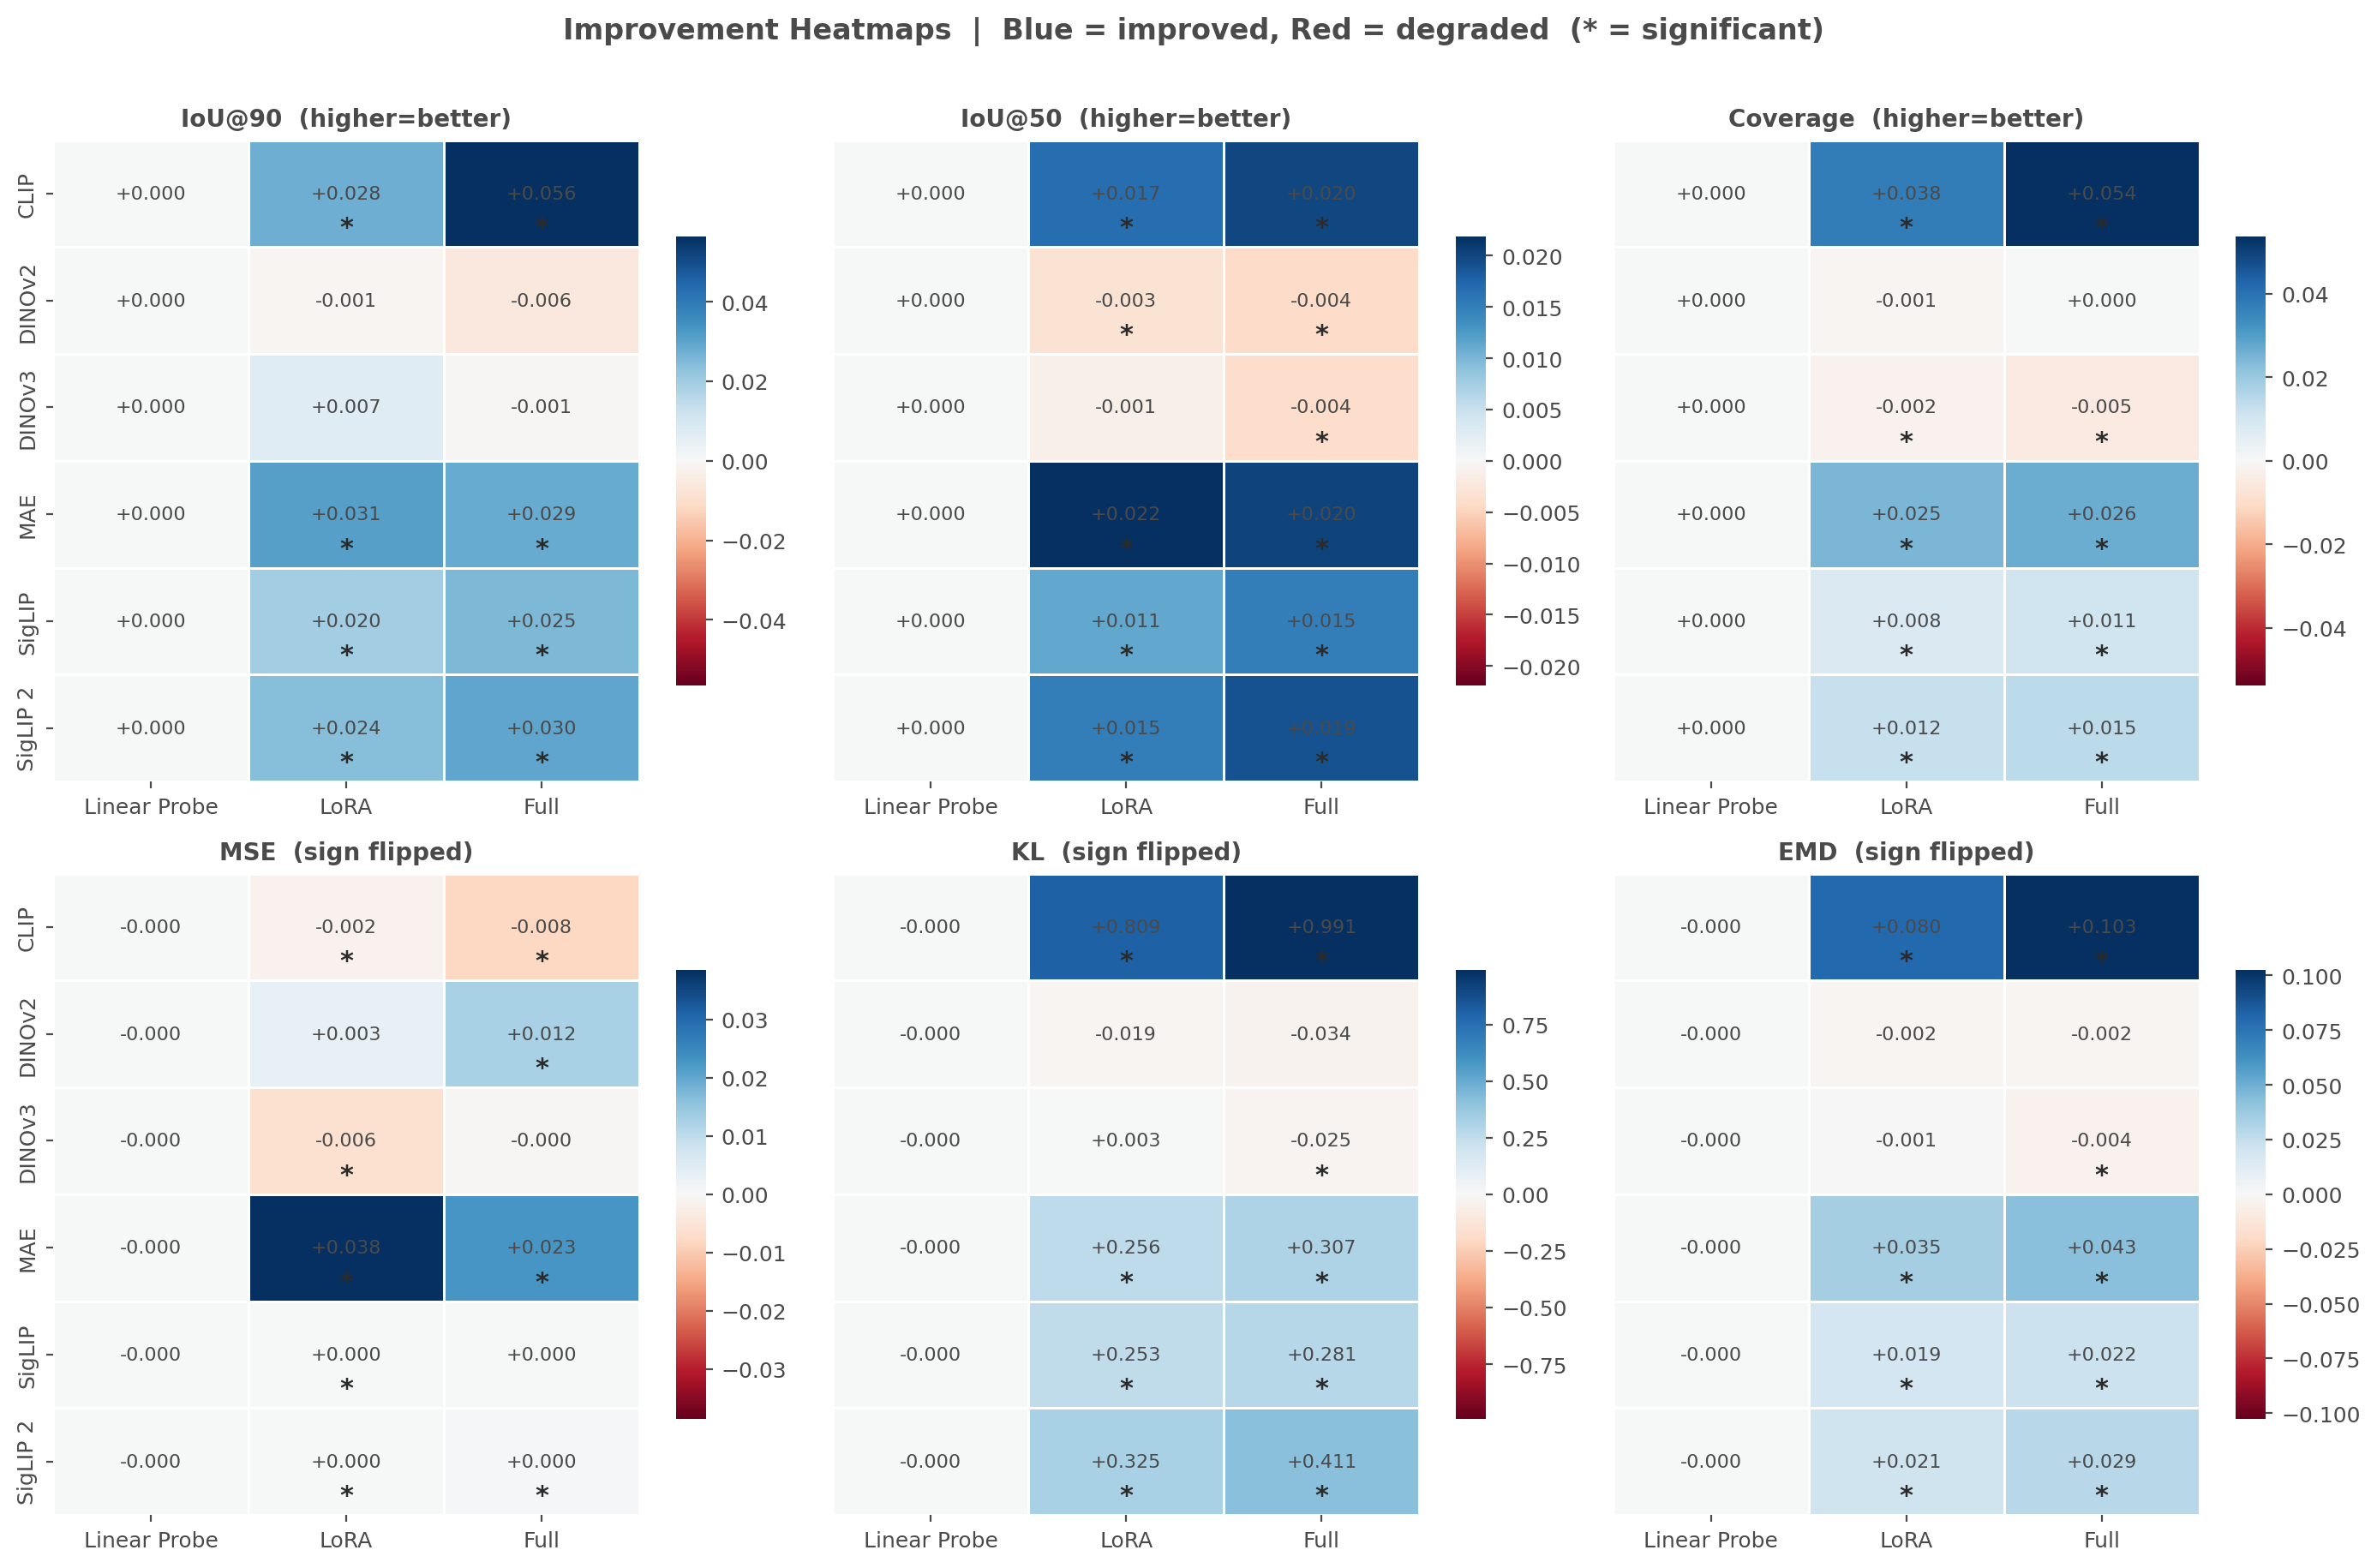
\includegraphics[width=\columnwidth]{02_all_metrics_improvement_heatmap.png}
  \caption{Q2 multi-metric improvement heatmap. Each cell shows whether LoRA or Full fine-tuning enhances, preserves, or degrades alignment relative to the frozen model.}
  \label{fig:heatmap}
\end{figure}

\textbf{CLIP} shows the largest gain (Full fine-tuning: IoU $0.0181\!\to\!0.0745$,
Coverage $0.051\!\to\!0.105$, Cohen's $d\!\approx\!1.0$). The per-style
breakdown (Table~\ref{tab:perstyle}) reveals that virtually all of CLIP's gain
concentrates on Romanesque (+0.066) and Gothic (+0.079) images, whose diagnostic
features (Round Arch Portals, Pointed Arch Portals, Tracery) appear frequently
in English-language web text---consistent with CLIP's language-grounded training.
Renaissance (+0.014) and Baroque (+0.013) show near-zero gain.

\begin{table}[h]
\caption{Per-style $\Delta$IoU@90 under Full fine-tuning (frozen~$\to$~fine-tuned).}
\label{tab:perstyle}
\centerline{\small
\begin{tabular}{lcccc}
\toprule
Model & Roman. & Gothic & Renaiss. & Baroque \\
\midrule
CLIP    & +0.066 & +0.079 & +0.014 & +0.013 \\
MAE     & +0.014 & +0.011 & +0.108 & +0.001 \\
SigLIP2 & +0.038 & +0.041 & +0.022 & +0.009 \\
SigLIP  & +0.031 & +0.035 & +0.018 & +0.007 \\
DINOv2  & +0.002 & +0.001 & $-$0.003 & $-$0.001 \\
DINOv3  & +0.001 & $-$0.002 & $-$0.005 & $-$0.003 \\
\bottomrule
\end{tabular}
}
\end{table}

A Kruskal-Wallis test finds significant style moderation for CLIP
($p\!=\!7.2\!\times\!10^{-9}$), MAE ($p\!=\!3.8\!\times\!10^{-7}$), SigLIP
($p\!=\!1.5\!\times\!10^{-5}$), and SigLIP2 ($p\!=\!5.0\!\times\!10^{-7}$);
DINOv2 and DINOv3 are not significant ($p\!=\!0.18$, $p\!=\!0.12$), consistent
with their near-zero per-style profiles.

\textbf{MAE}'s Renaissance $\Delta$ of +0.108 is the largest single-style shift
in the dataset. Table~\ref{tab:mae_renaissance} shows this gain is concentrated
on pediment-class features, which are geometrically compact and
Renaissance-exclusive. The two most common Renaissance features (Pilaster,
Belt Course) show negative $\Delta$, suggesting the style-classification gradient
routes attention toward the most discriminative geometric forms.

\begin{table}[h]
\caption{Per-feature $\Delta$IoU for MAE (Full fine-tuning, Renaissance images).}
\label{tab:mae_renaissance}
\centerline{\small
\begin{tabular}{lccc}
\toprule
Feature & Froz.\ IoU & FT IoU & $\Delta$IoU \\
\midrule
Triangular Pediment & 0.003 & 0.083 & +0.080 \\
Cranked Cornice     & 0.002 & 0.064 & +0.062 \\
Broken Pediment     & 0.001 & 0.056 & +0.055 \\
Volute              & 0.004 & 0.047 & +0.043 \\
Segmental Pediment  & 0.002 & 0.044 & +0.042 \\
Pilaster            & 0.031 & 0.019 & $-$0.012 \\
Belt Course         & 0.027 & 0.011 & $-$0.016 \\
\bottomrule
\end{tabular}
}
\end{table}

\textbf{DINO family:} Both DINOv2 and DINOv3 show near-zero $\Delta$ across all
styles and strategies. $\Delta\!\approx\!0$ is a positive generalisation result:
expert-aligned spatial structure is already encoded by pretraining, and the
style-classification gradient is absorbed by the classification head rather than
reshaping backbone attention.

Figure~\ref{fig:ped} shows the preserve/enhance/destroy classification across
72 non-Linear-Probe model$\times$strategy$\times$metric combinations: 46 enhance,
16 preserve, 10 destroy. Figure~\ref{fig:forest} adds the statistical layer with
bootstrap confidence intervals.

\begin{figure}[t]
  \centering
  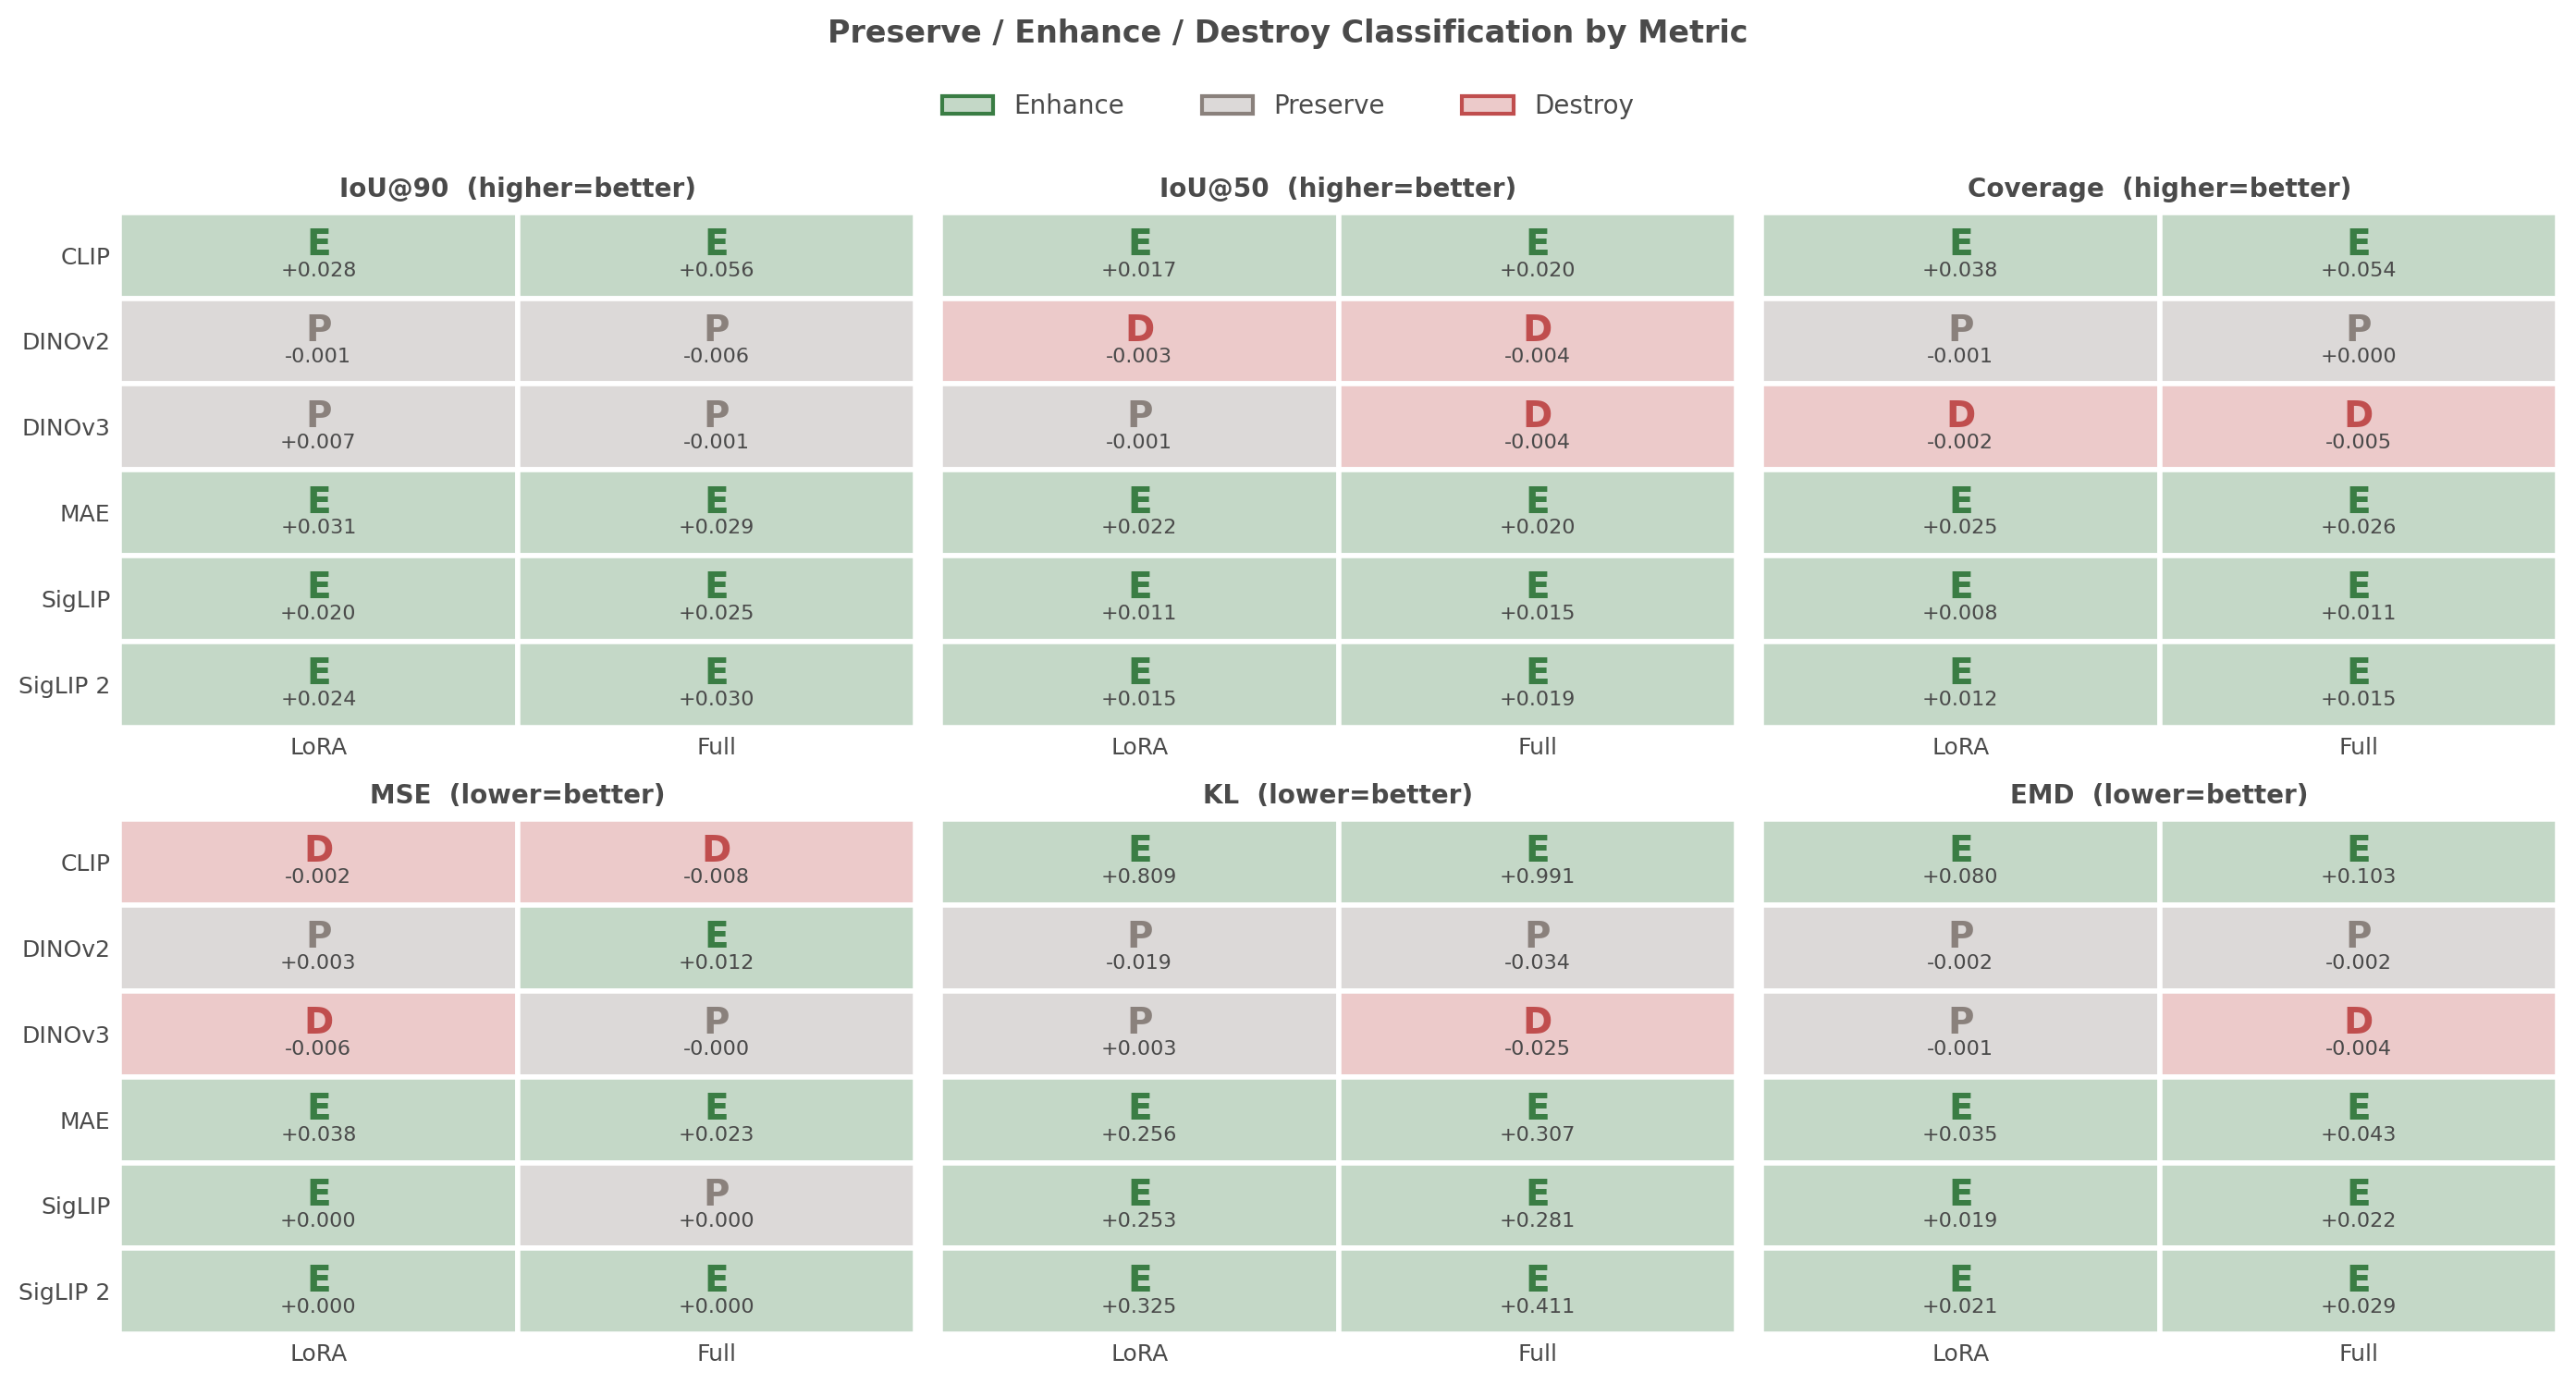
\includegraphics[width=\columnwidth]{07_preserve_enhance_destroy.png}
  \caption{Preserve/enhance/destroy classification across 72 non-LP combinations. Fine-tuning dominantly enhances alignment, with concentrated regression risk.}
  \label{fig:ped}
\end{figure}

\begin{figure}[t]
  \centering
  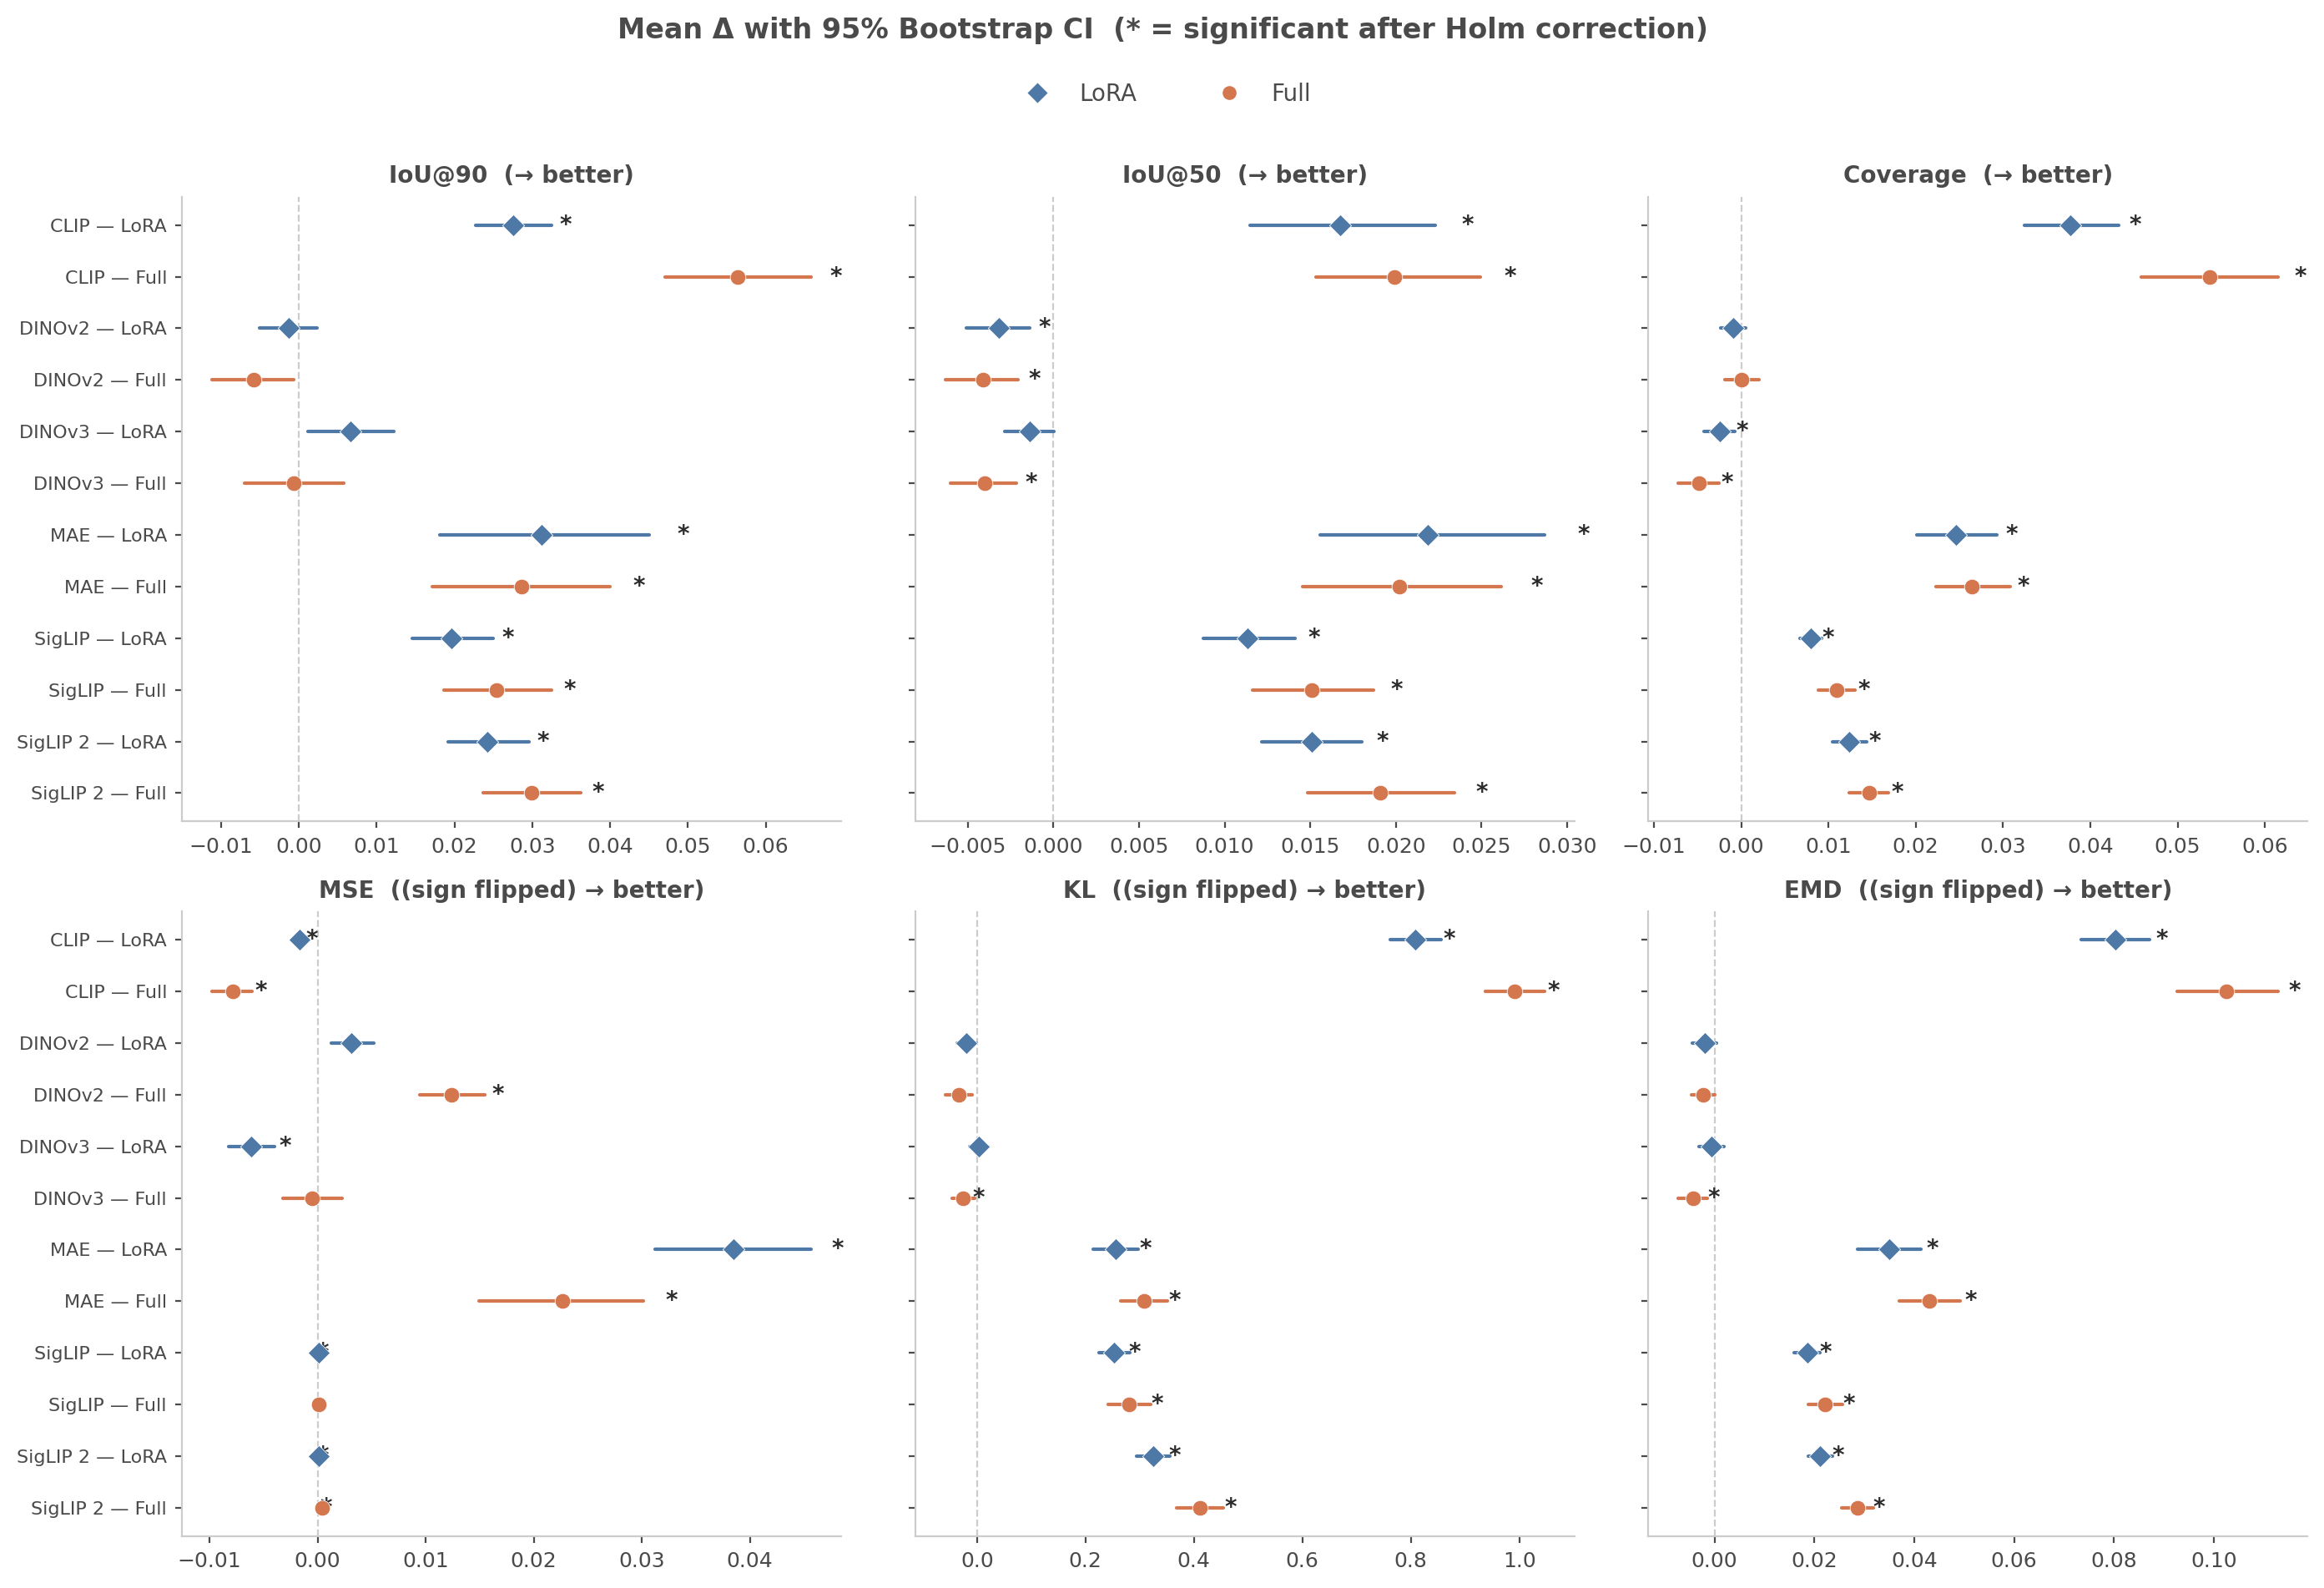
\includegraphics[width=\columnwidth]{08_forest_plot_ci.png}
  \caption{Forest plot of $\Delta$IoU@90 with 95\% bootstrap confidence intervals per model and strategy.}
  \label{fig:forest}
\end{figure}

\textbf{Cross-model correlation.} DINOv3 frozen IoU predicts CLIP $\Delta$IoU
at Pearson $r\!=\!+0.677$ ($\rho\!=\!+0.681$, $p\!<\!0.0001$; see
Figure~\ref{fig:scatter}): the images CLIP gains on are the same structurally
easy images DINOv3 already attends to. Within-cluster language-model
correlations (CLIP--SigLIP--SigLIP2) are $r\!\approx\!0.43$--$0.58$; MAE is
anti-correlated with the language cluster ($r\!\approx\!{-}0.22$ to ${-}0.31$).
Models with different pretraining objectives converge on the same structurally
easy images rather than specialising on complementary subsets.

\begin{figure}[t]
  \centering
  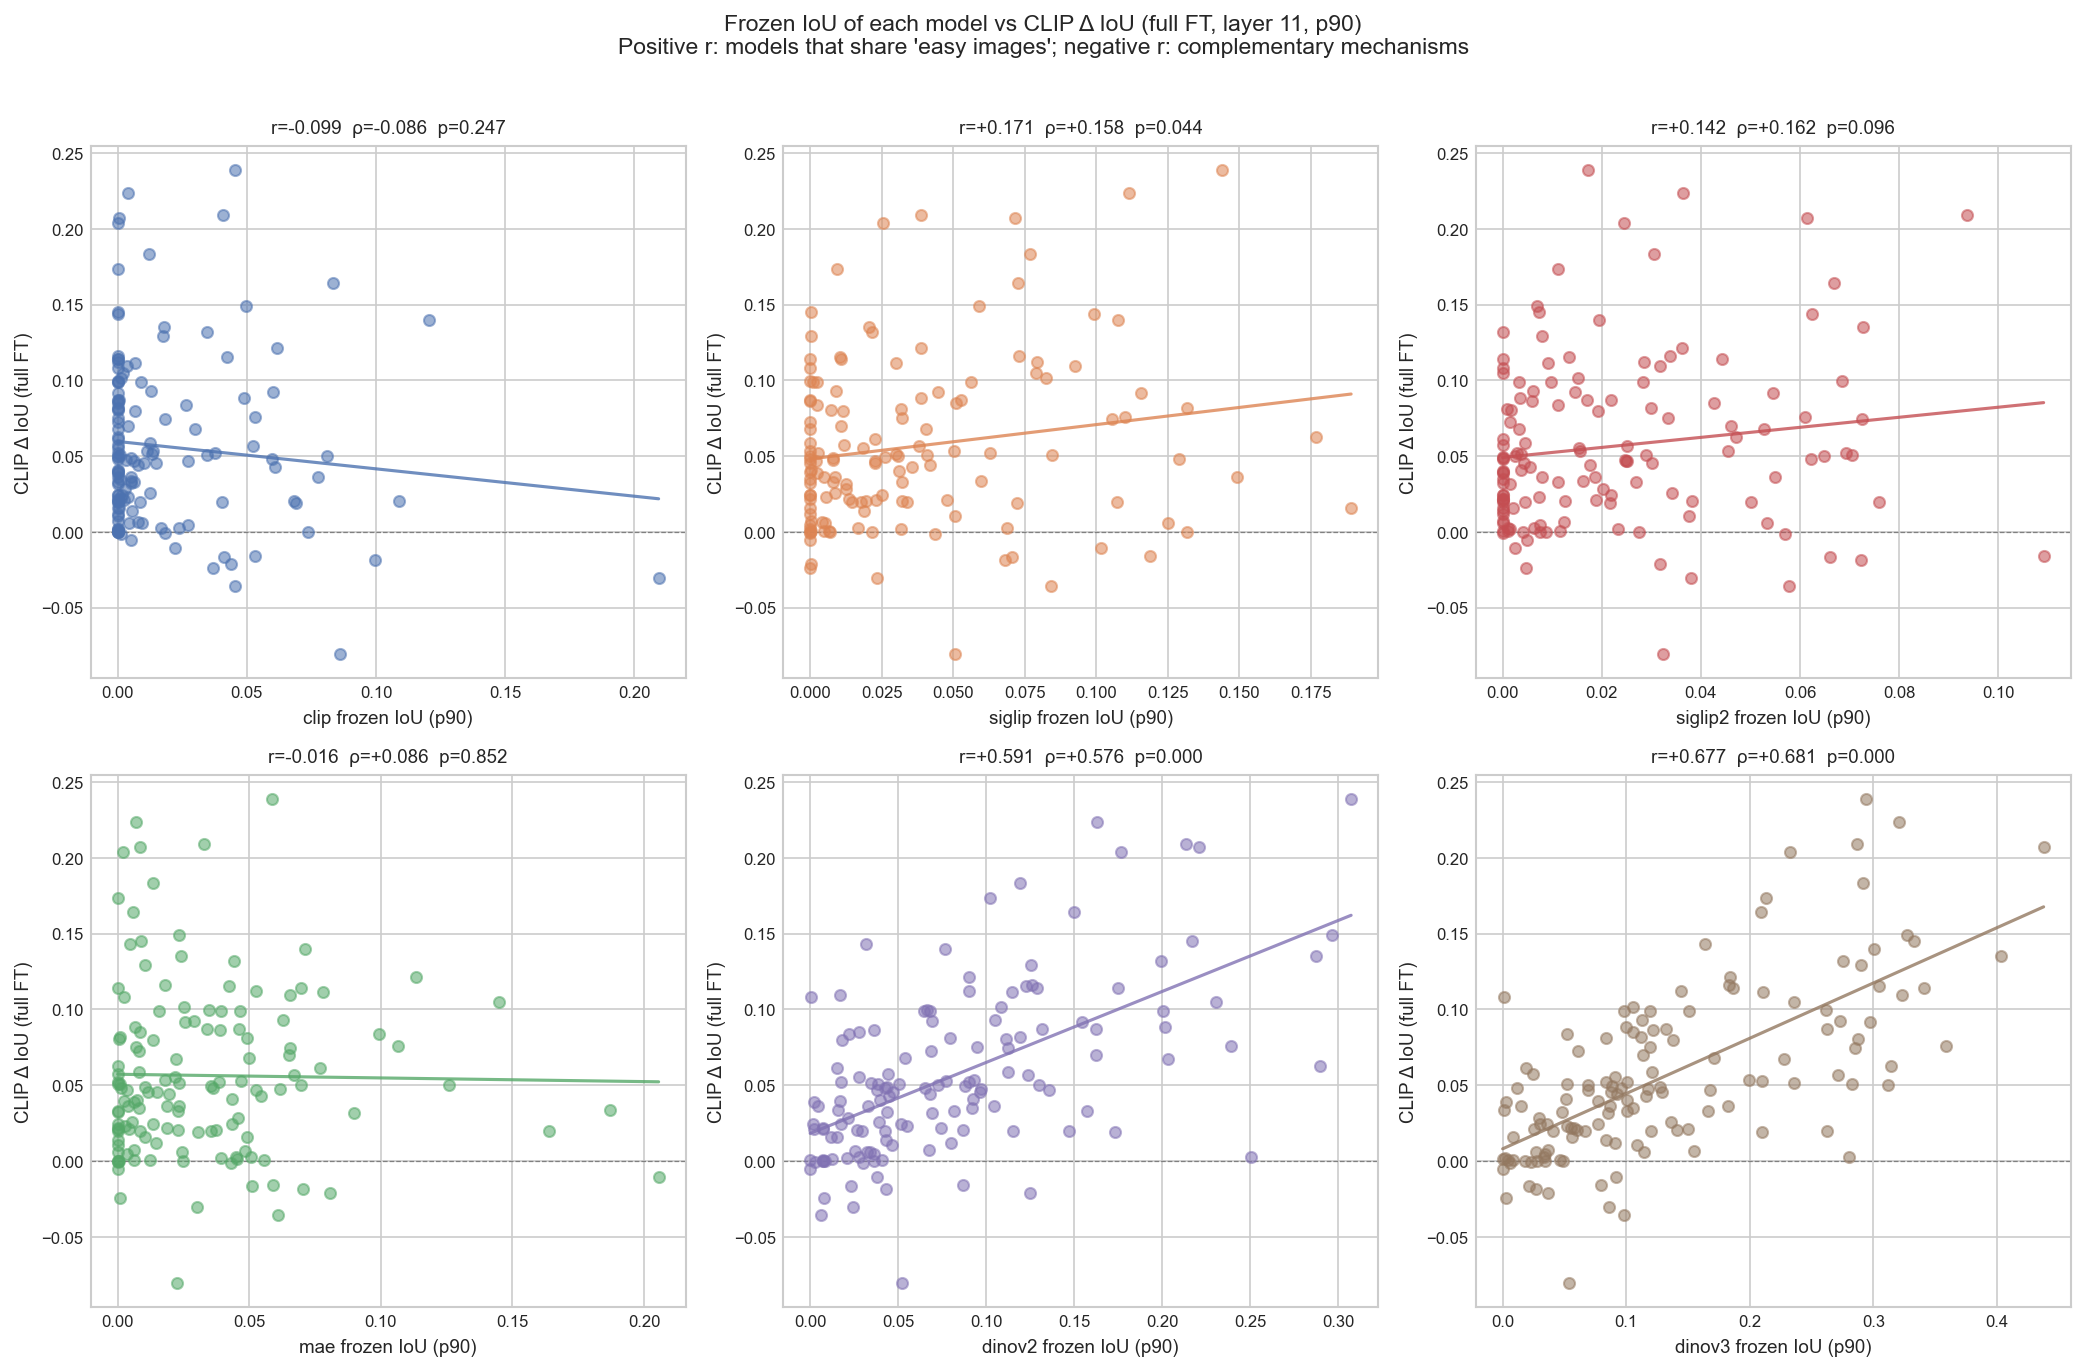
\includegraphics[width=0.85\columnwidth]{model_correlation_scatter.png}
  \caption{DINOv3 frozen IoU@90 vs.\ CLIP $\Delta$IoU@90 per image ($r\!=\!+0.677$). Structural image difficulty, not model family, determines what is ``easy''.}
  \label{fig:scatter}
\end{figure}

\subsection{Q3: Per-Head Specialisation}
\label{sec:q3}

Q3 analyses whether individual attention heads in DINOv2, DINOv3, MAE, and CLIP
exhibit descriptive specialisation for different architectural feature types
across frozen, LoRA, and Full variants.

% TODO: Insert final Q3 head-ranking figure (source: outputs/cache/metrics.db, per_head tables).
% TODO: Insert finalized Q3 narrative once scoped head-specialisation claims are confirmed.

The current pipeline supports per-head IoU ranking, head-by-feature alignment
matrices, and per-image exemplar storage. The primary analysis will report
whether late-layer head dominance is sparse, whether supervision family changes
the dominant head set, and whether LoRA or Full fine-tuning shifts dominant
heads relative to frozen.

\subsection{Ablation Study: Preserve / Enhance / Destroy}

The preserve/enhance/destroy classification in Figure~\ref{fig:ped} serves as
the primary ablation across the full model$\times$strategy$\times$metric matrix.
Key findings: (1)~Linear Probe is a true zero-change control across all models;
(2)~Full fine-tuning produces the most enhance outcomes overall but also the most
destroy outcomes for already-aligned models; (3)~LoRA captures a substantial
share of Full fine-tuning's improvement while producing fewer regression cases
for the DINO family.

\subsection{Discussion and Limitations}

\textbf{Intuitive findings.} Linear Probe as a true attention-change control
validates that Q2 movement reflects representation change, not a reporting
artefact. Stronger task-conditioned adaptation helps most when the frozen model
is not yet strongly aligned---CLIP, MAE, and SigLIP-family results fit this
pattern.

\textbf{Surprising findings.} The SigLIP family pairs excellent frozen MSE with
EMD worse than random, illustrating why single-metric interpretation is
dangerous. DINOv2 does not improve dramatically under Q2 despite other families
gaining substantially: self-distillation may already produce more part-like
spatial attention, leaving less headroom for downstream adaptation.

\textbf{Pretraining objective account.} CLIP's InfoNCE loss~\cite{Radford21CLIP}
applies no patch-level spatial pressure; fine-tuning is the first spatial signal,
and the gain concentrates on styles whose features are linguistically described.
MAE's 75\%-masking objective~\cite{He22MAE} forces precise local geometry
representations, which explains its Renaissance pediment affinity. DINOv3's
Gram-anchoring loss~\cite{Simeoni25DINOv3} explicitly preserves second-order
spatial structure, explaining its $\Delta\!\approx\!0$ result under Q2.

\textbf{Practical implications.} Model selection for domain adaptation should
not be guided by accuracy alone. DINOv3 may be preferable when plausible
evidence use matters without adaptation; CLIP or MAE become more attractive when
adaptation is allowed. LoRA captures most of the attention-shift benefit in
several models with fewer regressions than Full fine-tuning. MAE is the only
model whose per-image $\Delta$ is anti-correlated with the language cluster,
making it the natural complementary partner in coverage-seeking ensembles.

\textbf{Limitations.} The annotated evaluation subset is small (139 images),
limiting statistical power. Bounding boxes are expert-guided but not exhaustive,
introducing sparse annotation bias especially for Baroque. Attention is an
incomplete explanation signal: strong alignment is evidence of plausibility, not
causal proof. IoU depends on the thresholding rule; continuous metrics require
calibration to avoid overreading raw numbers.

% -----------------------------------------------------------------------
\section{Conclusions and Future Work}
\label{sec:conc}

This project asks whether self-supervised vision models attend to the same
architectural evidence that experts consider diagnostically important. Using
WikiChurches, expert bounding boxes, and a multi-metric alignment framework, we
address three linked questions across seven models and three fine-tuning
strategies.

For \textbf{Q1}, frozen expert-aligned attention exists but is not evenly
distributed. DINOv3 provides the strongest evidence, leading the default-method
benchmark on IoU, Coverage, KL, and EMD and clearing all calibrated baselines.
The safest interpretation is not that all SSL models attend like experts, but
that DINOv3's spatial prior is unusually compatible with expert-marked
architectural evidence in WikiChurches.

For \textbf{Q2}, fine-tuning's effect is mediated by three interacting factors:
the pretraining objective's spatial prior (DINO preserves strong frozen
alignment; CLIP, MAE, and SigLIP-family gain because they lack it); dataset
linguistic coverage (CLIP's gain concentrates on Gothic and Romanesque features
densely described in English web text); and geometric discriminability (MAE
redirects attention to Renaissance-exclusive pediment forms that pixel
reconstruction already encodes with high local fidelity). Models with different
objectives converge on the same structurally easy images rather than
complementary subsets, with implications for ensembling strategies.

For \textbf{Q3}, the per-head specialisation pipeline is in place and the
analysis scope is defined. Final findings will be reported once the per-head
claim set is confirmed.

\textbf{Future work.} A patch-level text-similarity probe for CLIP would
directly test the linguistic-grounding hypothesis. Extending the annotated pool
beyond 139 images would improve statistical power and reduce Baroque annotation
sparsity. A Gram-anchoring ablation on DINOv3 would isolate whether the spatial
prior is driven by data scale, model scale, or the anchoring loss specifically.

% -----------------------------------------------------------------------
\section{Author Contributions}

\textbf{Desmond Choy}: project lead, fine-tuning pipeline, Q2 analysis, result
interpretation, system architecture and backend.

\textbf{Leong Kay Mei}: frontend and analysis interface, precompute pipeline,
metric design and validation, Q1 calibration, documentation.

Both authors contributed to research design, experiment execution, and report
writing.

% -----------------------------------------------------------------------
\section{AI Tool Declaration}

The authors used Claude (Anthropic) to [describe specific uses: e.g., assist
with literature review summaries, improve expression, format LaTeX, generate
draft text for revision]. The authors are responsible for the content and
quality of the submitted work.

% -----------------------------------------------------------------------
\bibliographystyle{IEEEbib}
\bibliography{references}

% -----------------------------------------------------------------------
\appendix
\section*{Appendix A: Structurally Easy vs.\ Hard Images}

Each row shows one representative church from the annotated evaluation set. Left:
DINOv3 frozen CLS attention at layer~11 with expert boxes overlaid. Centre: CLIP
frozen-vs-fine-tuned shift map (blue~=~gained, red~=~lost attention). Right:
shift map with selected expert feature box highlighted.

\begin{figure*}[t]
  \centering
  % Row 1: Easy -- Gothic
  \begin{subfigure}[t]{0.16\textwidth}
    \includegraphics[width=\linewidth]{{Q1710328_DINO__EASY(gothic)}.png}
    \caption*{\small DINOv3 frozen}
  \end{subfigure}\hfill
  \begin{subfigure}[t]{0.16\textwidth}
    \includegraphics[width=\linewidth]{{Q1710328_CLIP_DELTA__EASY(gothic)}.png}
    \caption*{\small CLIP shift}
  \end{subfigure}\hfill
  \begin{subfigure}[t]{0.16\textwidth}
    \includegraphics[width=\linewidth]{{Q1710328_CLIP_DELTA_IMG__EASY(gothic)}.png}
    \caption*{\small Feature box}
  \end{subfigure}\hfill
  % Row 1: Easy -- Romanesque
  \begin{subfigure}[t]{0.16\textwidth}
    \includegraphics[width=\linewidth]{{Q2034923_DINO__EASY(romanesque)}.png}
    \caption*{\small DINOv3 frozen}
  \end{subfigure}\hfill
  \begin{subfigure}[t]{0.16\textwidth}
    \includegraphics[width=\linewidth]{{Q2034923_CLIP_DELTA__EASY(romanesque)}.png}
    \caption*{\small CLIP shift}
  \end{subfigure}\hfill
  \begin{subfigure}[t]{0.16\textwidth}
    \includegraphics[width=\linewidth]{{Q2034923_CLIP_DELTA_IMG__EASY(romanesque)}.png}
    \caption*{\small Feature box}
  \end{subfigure}

  \vspace{4pt}
  \textbf{Easy images} (high DINOv3 frozen IoU, high CLIP $\Delta$IoU).
  Q1710328 Gothic: DINOv3 IoU~$=$~0.438; CLIP $\Delta$IoU~$=$~+0.207 (Ornate Portal).
  Q2034923 Romanesque: DINOv3 IoU~$=$~0.403; CLIP $\Delta$IoU~$=$~+0.135 (Ornate Portal).

  \vspace{6pt}
  % Row 2: Hard -- Baroque
  \begin{subfigure}[t]{0.16\textwidth}
    \includegraphics[width=\linewidth]{{Q694252_DINO__HARD(baroque)}.png}
    \caption*{\small DINOv3 frozen}
  \end{subfigure}\hfill
  \begin{subfigure}[t]{0.16\textwidth}
    \includegraphics[width=\linewidth]{{Q694252_CLIP_DELTA__HARD(baroque)}.png}
    \caption*{\small CLIP shift}
  \end{subfigure}\hfill
  \begin{subfigure}[t]{0.16\textwidth}
    \includegraphics[width=\linewidth]{{Q694252_CLIP_DELTA_IMG__HARD(baroque)}.png}
    \caption*{\small Feature box}
  \end{subfigure}\hfill
  % Row 2: Hard -- Renaissance
  \begin{subfigure}[t]{0.16\textwidth}
    \includegraphics[width=\linewidth]{{Q1424095_DINO__HARD(renaissance)}.png}
    \caption*{\small DINOv3 frozen}
  \end{subfigure}\hfill
  \begin{subfigure}[t]{0.16\textwidth}
    \includegraphics[width=\linewidth]{{Q1424095_CLIP_DELTA__HARD(renaissance)}.png}
    \caption*{\small CLIP shift}
  \end{subfigure}\hfill
  \begin{subfigure}[t]{0.16\textwidth}
    \includegraphics[width=\linewidth]{{Q1424095_CLIP_DELTA_IMG__HARD(renaissance)}.png}
    \caption*{\small Feature box}
  \end{subfigure}

  \vspace{4pt}
  \textbf{Hard images} (low DINOv3 frozen IoU, low CLIP $\Delta$IoU).
  Q694252 Baroque: DINOv3 IoU~$=$~0.000; CLIP $\Delta$IoU~$=$~$-$0.005 (Broken Pediment, peripheral).
  Q1424095 Renaissance: DINOv3 IoU~$=$~0.002; CLIP $\Delta$IoU~$=$~+0.002 (spatially diffuse annotations).

  \caption{Appendix A: Structurally easy (top) and hard (bottom) church images.
  The $r\!=\!+0.677$ correlation between DINOv3 frozen IoU and CLIP $\Delta$IoU
  shows that image structure, not model family, determines alignment difficulty.}
  \label{fig:appendix_a}
\end{figure*}

\end{document}
